\documentclass[pdftex,12pt]{llncs}
  \usepackage[american]{babel}
  \usepackage{fullpage}
  \usepackage{wrapfig}
%  \newcommand{\x}[1]{ }
  % This is where the bibliography stuff needs to happen
  \usepackage[style=apa,backend=biber]{biblatex}
  \DeclareLanguageMapping{english}{american-apa}
  \addbibresource{billTolls.bib}
  \addbibresource{Projects-garbageCanCongress.bib}
  \usepackage[utf8]{inputenc}
  \usepackage{csquotes} % context sensitive quotes ---makes this look good
  \usepackage[pdftex]{graphicx}
  \usepackage{xfrac}
  \usepackage{cleveref}


\begin{document}

\title{For Whom the Bill Tolls}
\subtitle{A Simulated Annealing Model of Draft Legislation in Congress}
%\titlerunning{}
\author{Scott Atherley \and Clarence Dillon \and Vince Kane}
\institute{George Mason University\\
 \thanks{We wish to thank Maksim Tsvetovat who introduced us to the garbage can model in his course on Computational Organizational Theory and inspired us to extend it, adapt it, and to think about organizations and processes where it seems to fit especially well.}
% \email{satherle@gmu.edu \and cdillon2@gmu.edu \and vkane2@gmu.edu}}
  \email{\{satherle, cdillon2, vkane2\}@gmu.edu}}

\maketitle

\begin{abstract}
 We are interested in how network types can impact productivity of legislatures. 
 We apply a simulated annealing process in an agent-based model to modify draft legislation with legislator's priority issues in peer and committee reviews before a floor vote determines a congress's approval for a bill.
 The model design enabled extensive experimentation and we present an overview of the most significant insights. We found that having exogenous, common issue priorities has a high impact on productivity but that some structures inhibit productivity.
\end{abstract}

\section{Introduction}
The dynamics of policy-making in Congress have been extensively studied. 
Numerous formal and empirical models of various aspects of the institution have been developed and tested, including: voting decisions \parencite{m74, k89}, Congressional ideology \parencite{pr97}, party influence in Congress \parencite{cm93,cm05,a95} or lack thereof \parencite{k91, k98} and committee dynamics \parencite{sw87, gk89, m04}. 
In spite of this wealth of literature there remains surprisingly little research on the precise dynamics of policy formation. 
Existing models tend to reason backwards from votes: constructing measures of ideology from grouped voting decisions, assuming that legislators devise legislation that aligns with their past voting patterns.  

This research complements these studies by developing a model of policy development through draft legislation. 
We model the development of legislation as a sequential bargaining process among sub-groups within the Congress. 
An initial round of informal consideration among colleagues forms the basis of a formally introduced bill; reflecting a search for cosponsors. 
Cosponsors alter the draft before `signing-on' and add information (and preferences) to the legislation. 
We model this process with a simulated annealing algorithm, representing legislation and preferences as bit string attributes. 
After the initial round of annealing generates an outcome---the \textit{draft legislation}---a second round of annealing---\textit{committee consideration}---ensues. 
Finally, our simulated Congress votes on the issue.

Taking this approach to the policy-making process captures several crucial features of Congress that are often neglected. 
First, we model Congress as a networked body and treat bill-drafting as an essentially social process. 
Legislators seek out support from among their companions, selected primarily by homophily. 
Second, we explicitly model the role of draft legislation and informal policy-making groups in Congress. 
This form of policy-making has been prominent recently, with various ``gangs'' of legislators emerging to formulate draft solutions.

The model produces insights about the network structures that are consistently more productive. The model also shows the ideological conditions under which Congress can be most productive. 
        

\section{Networks and Policy Choice in Congress}
%\textquote[Morgan2009,10]{how they function as \textit{instruments} of investigation}.

Congressmen face many competing considerations in their role as legislators. 
They must balance their constituents against interest groups and struggle to form make correct policy choices in the face of broad uncertainty. 
This paper addresses the role of networks and draft bills in combating this uncertainty and creating viable legislation.
Legislators face a large body of colleagues with heterogeneous preferences. 
They also face serious consequences if they fail too publicly. 
As Thomas Mann once observed, Congressmen feel \textquote{unsafe at any [electoral] margin} \parencite{m78}. 
Moreover, social choice problems (\textit{e.g.}, \cite{sw87} severely complicate the emergence of any stable policy outcome. 
The structure of Congress is designed, in part, to mitigate these challenges\parencite{sw87}. 

There is a rich literature on agenda control devoted primarily to explaining how politics and power color the outcomes of legislative choice. 
Agenda control arguments run through committees, although researchers differ on how committees are formed and influenced. 
Partisan policy-making theories emphasize \textit{negative agenda control} over the legislative process: by dominating committees, parties prevent legislation they do not support from reaching the floor \parencite{cm93,cm05}.
Parties also wield \textit{positive agenda control}, the ability to push favored bills through the legislative process \parencite{r91,a95}. 
On the other hand, Krehbiel (1991, 1998) argues that committees are ultimately controlled by individual legislator preferences, and specifically the median member of the chamber in question (following the classic median voter theorem; \cite{b48}. 
While these theories have their differences, they share a keen awareness of the importance of institutional roles and powers in the legislature. 
The implication of both theories is that policy ought to change substantially as it moves through the legislative process---if committees act as gatekeepers, whether on behalf of their own particular interests, the House floor, or party leadership, they should possess the power to shift policy in the direction they desire.   

Both theories also suggest the importance of building support for legislation prior to formal consideration. 
Without some level of initial backing, either from party elites or an adequate subset of legislators on the floor, policy is highly likely to die in committee. 
Legislative productivity data reveals this trend clearly: Table \ref{billpassrate} charts the percentage of bills introduced that actually received a floor vote (see also footnote \ref{passfn}).

The vast majority of legislation goes to committee to die. 
A random piece of legislation, without co-sponsors or other forms of support, is unlikely to be an exception. 
The nature of the policy-process also suggests a strong value to establishing support for legislation early: given the power of entrenched forces (whether acting on behalf of party or preferences) at each step of a bill's progression through Congress a sponsor must carefully marshal a supporting coalition or risk his interests being completely overwhelmed by others.

\begin{wrapfigure}{l}{0.5\textwidth}
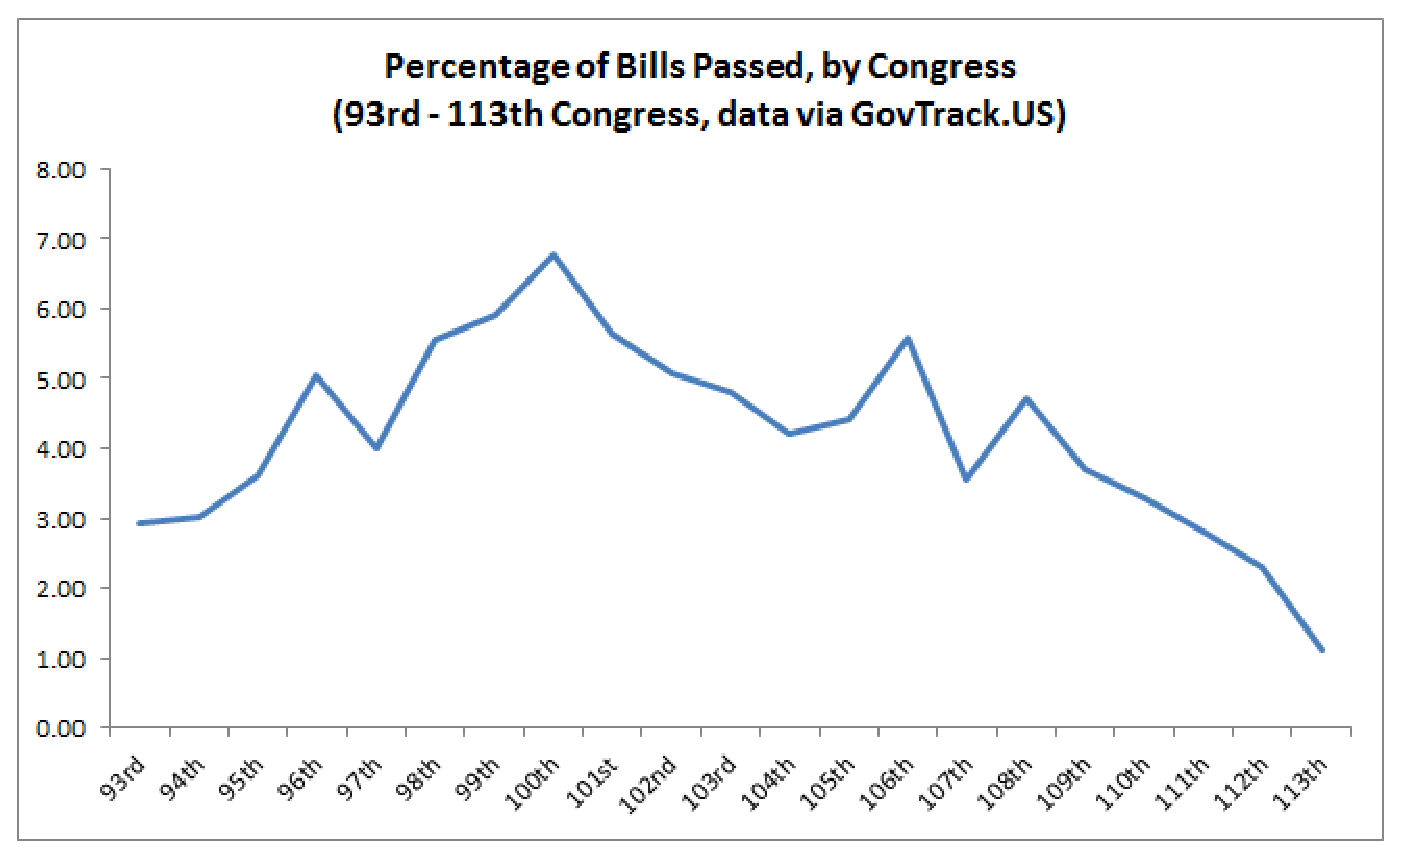
\includegraphics[width=0.49\textwidth]{percentPassed.eps}
\caption[ ]{Percentage of Bills Passed by Congress, $93^{rd}$ - $113^{th}$ Congress via \url{www.GovTrack.us}}
\label{billpassrate}
\end{wrapfigure}
   
How do legislators build an initial base of support for policy? 
Existing research suggests several mechanisms. 
First, legislators might discuss their ideas with others informally, or circulate draft legislation to other members as a means of \textit{feeling out} support for a particular policy. 
This is a good method of obtaining co-sponsor support as well---rather than introduce legislation and wait for others to read it, members are likely to seek out potential backers. 
There is limited existing research on draft circulation. 
Nourse and Schacter assess the draft process from a judicial law perspective, noting that drafts are generated primarily by staffers, lobbyists and professional drafters based on input from legislators; typically in the form of broad summary documents \parencite{ns02}. 
This is broadly consistent with research on lobbying strategies. 
Rather than attempt to persuade their enemies, lobbyists function as informational resources for their allies \parencite{hw90, hk98}. 
One of their informational roles is to generate draft legislation and policy ideas. 
These theories suggest that specific pieces of draft legislation will appeal to certain subsets of legislators. 
If legislators are hearing similar things from their resources they are likely to develop similar policy ideas and support similar legislation.  

Network ties between legislators may also contribute to the development of policy. Existing literature on co-sponsorship networks suggests that ties between legislators might serve as a powerful means of predicting vote outcomes. 
Several studies (\textit{e.g.} \cite{zftpfm08}) use network data to assess political polarization: findings are consistent with more conventional studies of Congressional ideology (\textit{e.g.} \cite{pr97}), indicating that polarization has increased over time, especially in the U.S. House of Representatives. 
Tam-Cho and Fowler find that Congress follows the pattern of a \textit{small-world network} \parencite{tf10}. 
Their research indicates that weak-ties enhance the likelihood of final passage for important legislation. 
Bratton and Rouse conduct a similar analysis of US state legislatures and attempt to evaluate the variables that influence tie-formation \parencite{br11}. 
They find that co-sponsorship activity is predicted by ideology, district-proximity, demographic homophily and network transitivity. 
This research explains the findings of network measures of polarization: ideology influences tie-formation, which in turn leads to the development of ideologically stratified networks. 
Analysis of networks in Congress reveals that co-sponsorship ties act as powerful predictors of coalition formation in the legislature. 
This in turn suggests that the careful cultivation of network ties is a path to power in Congress. 
We argue that legislators cultivate co-sponsorship relationships, in part, through interactions revolving around draft legislation.

\section{Simulated Annealing Model of Informal Draft Modifications}
This paper considers the role of informal deliberations in forming policy solutions.
We develop a theory of policy-making oriented around draft-legislation and pre-legislative coalition building.
Circulating draft legislation functions as a mechanism to build initial support for legislation in order to raise the odds of a bill's success. 
Furthermore, the dynamics of policy agendas suggest that legislators face a constrained set of problems. 
The objective of forming solutions through informal coalition building is to control the solution environment, developing a piece of legislation that addresses the relevant problem while also allowing other legislators to take advantage of the opportunity by adding their own solutions and issues of interest. 

The original bill sponsor, a legislator who has decided to attempt to make policy, is faced with a choice: should he distribute his policy proposal widely and attempt to solicit broad support? 
Or, should he keep distribution relatively restricted, retaining more certainty over content? 
We assume that once a policy is released it is largely removed from the sponsor's hands. 
Admittedly, this is not literally true: a sponsor can always withdraw legislation. 
However, we believe it is effectively true---even if a sponsor withdraws from legislation in response to substantial changes made by others, the other legislators may easily re-introduce new, equivalent legislation. 
In other words, the sponsor's primary role is to introduce a policy issue into the legislative arena and to propose a solution. 
The outcome of his action is left in the hands of his colleagues. 

There are recent examples of this form of informal, sub-group policy-making. 
Consider the various informal ``gangs'' of legislators that coalesced around competing solutions to the 2012-2013 budgetary crises, \textit{e.g.}, the \textit{Gang of 6}. 
These groups represent initial sub-sets of legislators considering draft legislation. 
In most cases they had no formal authority beyond some degree of respect from their peers. 
Ultimately, their proposed solution failed to become policy. 
This outcome was seen as a failure of bipartisanship and moderate politics. 
In contrast, we postulate that it could be a failure to understand the dynamics of informal policy-making. 
The \textit{Gang of 6} was too small to make an impact. 
While negotiation is easier among small groups, there is simply no guarantee that agreement among a small subset of a legislative body will translate into support within the entire body.

\section{Model Overview}
In this section, we present a model of informal policy formation based on simulated annealing. 
Conceptually, a bill is sponsored and considered by a network of legislators. 
This initial, informal group of policy-makers develops the framework of legislation through a round of annealing and builds some support for passage. 
Their work is then referred to a committee of interested members, who are allowed to alter the legislation through an additional round of annealing. 
This second alteration is analogous to committee agenda-setting powers \parencite{cm93, cm05}. 

Each realization of the simulation is initialized with a new group of legislators.  
These legislators have a list of priorities and positions associated with a list of issues. Legislator priorities and positions may or may not conform to an ideological party agenda, depending on model parameters. 
Finally, a social network connecting the legislators is generated, using both homophily \parencite{msc01, br11} and preferential attachment \parencite{Barabasi1999}.

\subsection{Model Processing}
The simulation sequentially repeats the following process for 200 proposals (or halts if all issues are passed into law): 

\begin{enumerate}
  \item Proposal:
  \begin{enumerate}
    \item A random legislator is chosen to sponsor a bill.
    \item The sponsor proposes a draft bill on any issue that has not already been addressed by law.
  \end{enumerate}
  \item Draft circulation among cosponsors:
  \begin{enumerate}
    \item All legislators connected to the sponsor in the social network are selected as cosponsors.
    \item The cosponsors revise the draft using simulated annealing; new issues may be added to the bill during the revision process and solutions on existing issues may change.
  \end{enumerate}
  \item Committee review:
  \begin{enumerate}
    \item The draft is referred to a committee; committees are chosen according to legislators for whom the main issue of the bill is a high priority.
    \item The committee revises the bill by simulated annealing; again, new issues may be added and existing solutions changed as a result.
  \end{enumerate} 
  \item Floor vote:
    \begin{enumerate}
    \item The bill is referred to the floor for a vote.
    \item If the bill passes by simple majority (\textgreater 50\% votes), the bill is made into law; \textit{i.e.}, the solutions addressed by the bill are recorded and the issues may not be revisited for the remainder of the realization.
  \end{enumerate} 
\end{enumerate}

We implement the model in a Python simulation, with an object-oriented design. 
There are three high-level classes that interact in the model: \texttt{State}, \texttt{Legislator}, and \texttt{Bill}.  
We describe these further in separate sections below.
The fixed and free parameters of the model are listed and described in the Technical Appendix.

\subsection{Implementation Details} 
The implementation of the model proceeds in several major steps comprising the main interaction-loops of the model:  

\begin{description}
  \item[First] the model environment (\texttt{State}) initializes, establishing core parameter values.
  \item[Second] the simulation generates legislators within the model environment, drawing on key environmental variables. 
  \item[Third] the simulation generates a network among legislators, mapping them to friends within the environment.
  \item[Finally] the simulation develops a bill-proposal structure.
\end{description}


\subsubsection{Initialize Model Environment \texttt{state}}
The first procedure launched in the model is initialization of the \texttt{state} object. 
This object serves as the foundation for the subsequent generation of interacting components. 
The state defines a set of possible priorities for legislators, defines `party-platform' issues and establishes the associated priorities and positions. 
The environment creates the legislator agents, who are assigned a party affiliation and provided with a seeded priorities list and a set of issue positions. 
These seeds serve as the foundation for a later stochastic process of finalizing legislators' preferences on issues.  

\subsubsection{Generate Positions and Priorities}
Having established the environment, the model next generates legislator positions and priorities. 
Each legislator's position priorities are stochastically assigned with a preferential attachment method to the seed values provided by the state object. (See the Technical Appendix for details.)  
This preferential attachment method generates a power law distribution of priorities, so that a legislator places very high priority on a small number of issues but low priority on most issues.  
Our use of the seeded priority issues list means that legislators have some correlation in priorities to the extent that their seed priorities are the same, but heterogeneity is introduced scholastically.

The end-result of this process is a set of legislator agents with unique policy preferences. 
These policy preferences are conditioned by party priorities and the seed-variable established by the model environment in Step 1. 
This procedure contributes to the realism of the model environment. 
Congressmen all have particular issues about which they care deeply and prioritize more highly. 
We believe the power-law distribution of issue priority strengths is a reasonable assumption to reflect this in the model.

The final component of preference generation involves an assumption that affiliated legislators adopt the positions of their party.
For our model, we assume that several core issues represent powerful, crystallizing factors that differentiate our simulated parties.  
We justify this assumption with existing research which indicates that legislator preferences generally reduce to a single dimension in the case of floor votes (Poole and Rosenthal 1997). 
For all other issues, positions are assigned randomly from the range $[0, 2^{Solution\_Bit\_Length} - 1]$, inclusive (\textit{i.e.}, a random bit string of a predefined length, set to the variable \texttt{solution\_bit\_length}).

\subsubsection{Network Generation}
Having generated an environment and a population of legislator agents with unique characteristics, we complete the model universe by generating a social network among legislators. 
This network is designed to capture the social dynamics of legislating, in that a Congressmen will naturally have a set of friends and close colleagues that he interacts with more than others. 

Drawing on legislator positions and priorities, we generate a social network using \textit{preferential-attachment} and homophily mechanisms.
Figure \ref{networkgeneration} depicts our process. 

\begin{wrapfigure}{l}{0.5\textwidth}
% \vspace{4.5cm}
  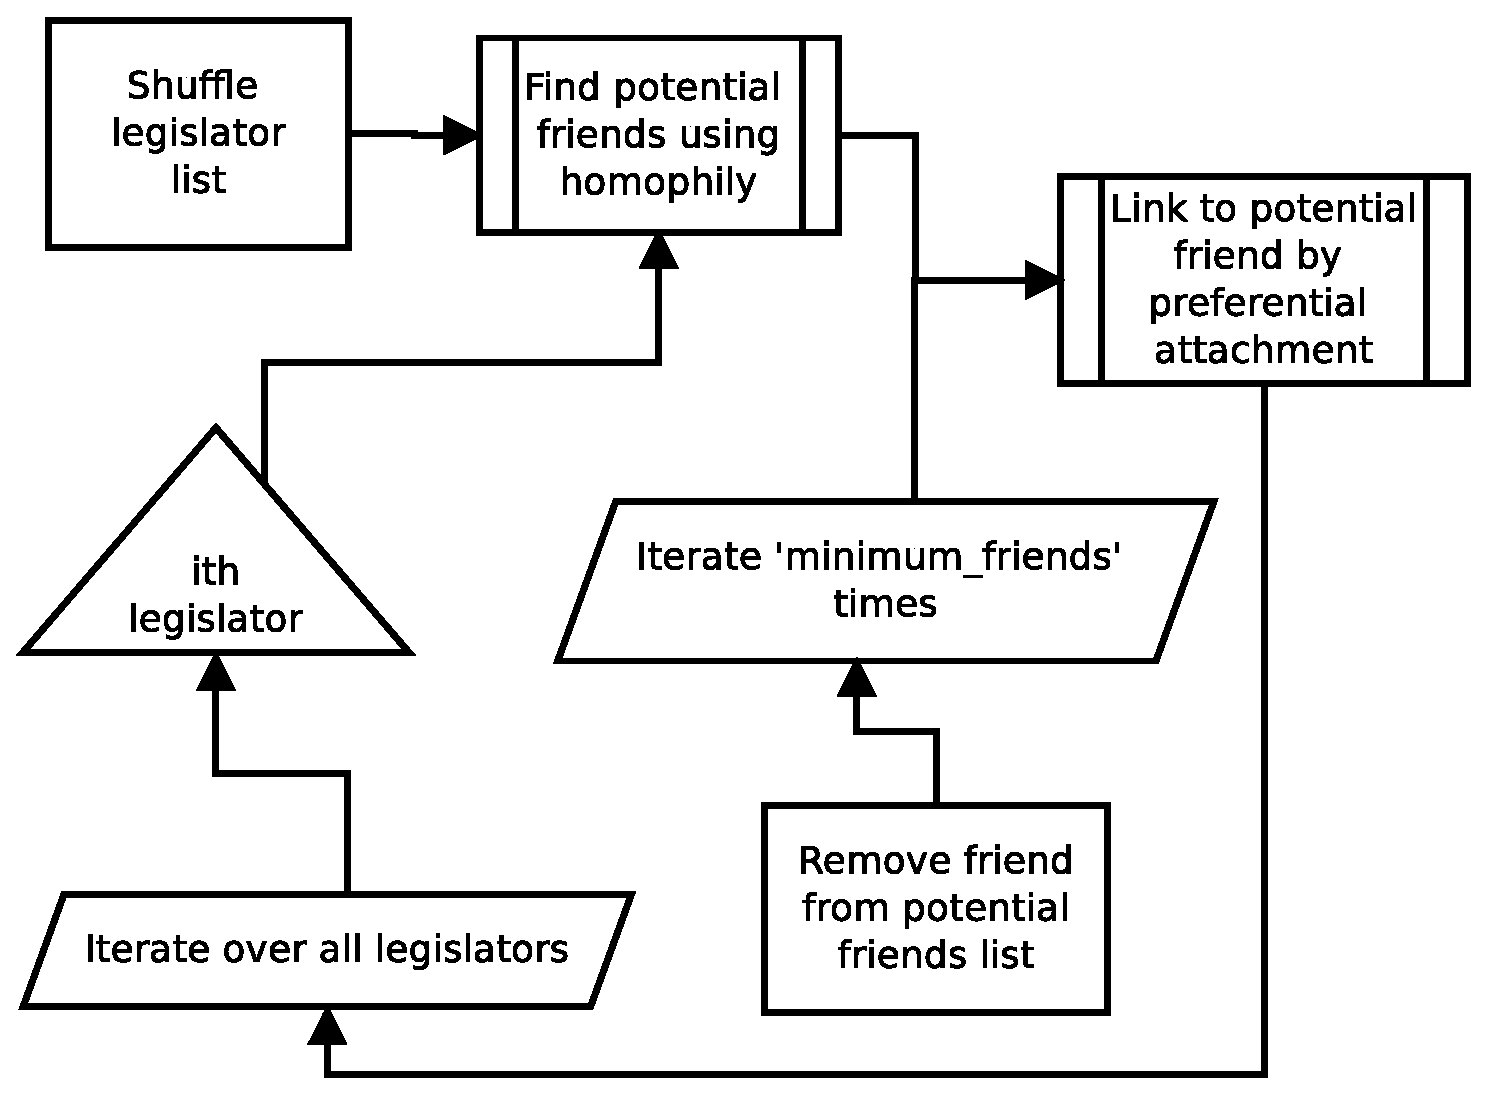
\includegraphics[width=0.48\textwidth]{networkProcess.eps}
 \caption[ ]{The network generation process}
 \label{networkgeneration}
\end{wrapfigure}

Homophily (similarity between two legislators) is the inverse of distance, which we calculate as the distance between two \texttt{issue} bit strings. 
We define distance as the increasing depth on a binary tree, where the most significant bit (MSB) of two bit strings is worth 50\% similarity, the next MSB is an additional 25 similarity, \textit{etc}.  
Two identical strings result in 100\% similarity, whereas strings that have only the MSB in common are only 50\% similar.    
Since our model only uses a bit string length of 4, the maximum achievable dissimilarity is 93.75\%.\footnote{At position $i$ in the bit strings, a bit's difference in the binary value results in an additional $(1/2)i + 1$ reduction in similarity. For an infinitely long bit string length, similarity in all positions but the MSB would result in a 50\% similarity as well.}

We use this method to enable strong issue-position correlation between party-affiliated legislators while still allowing for some heterogeneity among their positions. 
The research in this report does not use this feature because party platform positions are homogeneous among affiliated members along non-party affiliated positions. 
However, we included this feature as an extension in future work.

Another benefit to this method, however, is that on any given issue, it generates a bi-modal (rather than uniform) distribution of all legislator positions. 
In a completely uncorrelated population---a Congress of independents---a uniform significance of bits towards homophily created an extremely low likelihood of any two legislators having sufficient agreement over the entire solution space to meet any reasonable assumption of friendship threshold.  
The decreasing significance of the binary tree method is more reasonable in that it could be said to model any two legislators agreeing on the generalities of a solution to an issue---say, ``for'' or ``against''--- while perhaps differing on implementation details.  
This makes the network generation more tractable using reasonable assumptions of friendship threshold and eases implementation.

A legislator's potential friends are defined as the set of legislator agents who have a minimum similarity of a pre-set \textit{friend-threshold} total homophily on all issues with the legislator.  
Similarity is a sum of homophilies on positions of all issues, weighted by and normalized to the legislator's priorities on those issues. 
Homophily on an issue is the unary inverse $(1 - x)$ of the distance between legislators positions and priorities.
Edge assignment is as described in Barabasi and Albert (1999): each time an edge is added, a probability distribution (\textit{pdf}) is generated from the degree distribution in the sub-network of potential friends, and a target node for the edge is selected randomly from that \textit{pdf}. 
The typical outcome of this procedure is a \textit{small-world} network among legislator agents, consistent with existing research on social networks in Congress \parencite{Granovetter1978}. 

\begin{wrapfigure}{r}{0.5\textwidth}
% \vspace{4.5cm}
  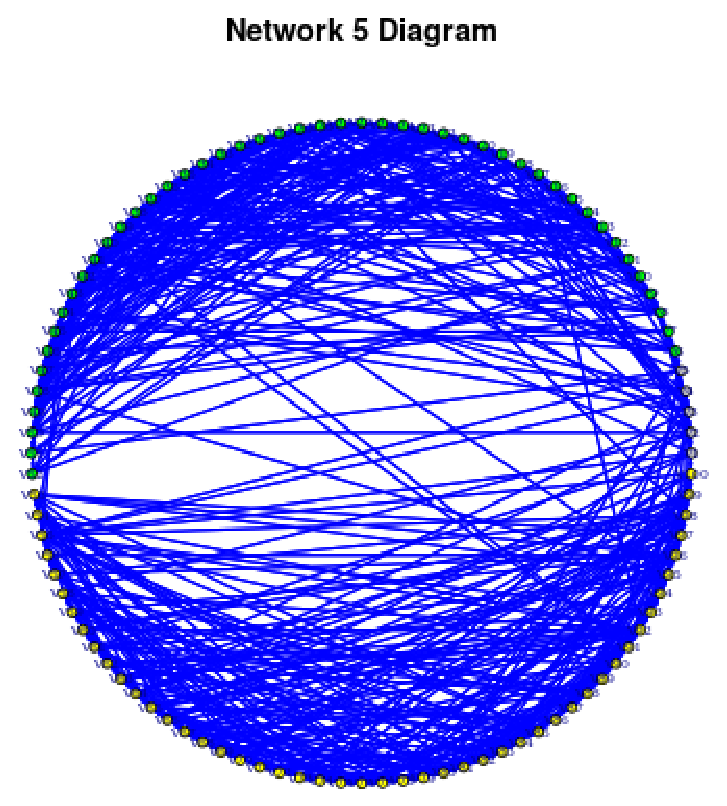
\includegraphics[width=0.48\textwidth]{smallworldnetwork.eps}
 \caption[ ]{`Network 5 Diagram' shows typical small-world properties in simple majority networks.  
Because the model generates network ties based on ideological homophily, the circular layout highlights a general division between Green (top half) and Yellow (bottom half) parties, with unaffiliated members (in grey, left side) more highly-connected to both Yellow and Green members.}
 \label{smallworldnetwork}
\end{wrapfigure}

\subsubsection{Bill Proposals}
Having defined a population of legislators and their relationship to each-other, we next establish a procedure for legislators to engage in the business of law-making.\footnote{One might argue that this is a departure from realism, as the current Congress does not appear to do this. However, we are attempting to generate a broadly generalizable model of law-making in legislatures. Some legislatures do legislate, periodically.} 
In our model, a sponsor is randomly selected to propose a piece of legislation. 
This legislation addresses a particular issue and he naturally sets his proposed solution to the issue at his preferred solution---his issue position. 
This process is analogous to ideal-point analysis in the Congress literature in political science \parencite{k98}. 

We innovate by going beyond basic proposals and counter-proposals. 
Once a sponsor develops a bill, he first initiates a search-process for co-sponsors, with the objective of building an initial base of support for his policy. 
This search phase coincides with a round of simulated annealing, discussed in the next sub-section. 
In brief, the bill is revised as co-sponsors join on. 
The sponsor gains support by sacrificing the purity of his positions; or, by adding additional issues and positions to the legislation, called ``bundling''.  

\subsubsection{Simulated Annealing}
The simulated annealer implements the Metropolis algorithm for simulated annealing \parencite{mrrt53, kgv}: a state with lower energy than the current state is accepted, while a state with higher energy is accepted with probability $P(state) = e^{\Delta E/kT}$.  
The annealer iterates over the temperatures provided to it in an annealing schedule and iterates a corresponding number of times provided to it for each temperature.  
At each iteration, a modifier function is called on the current state, the modified state's energy is calculated per the objective function, and the modified state's energy is then accepted or rejected.  
The final state returned by the algorithm is the lowest energy (highest satisfaction) state encountered.

For our model, we set $k$ to $k = -0.1/ln(1/2)$.  
This means that, at a temperature of $1.0$, a decrease of $0.1$ in satisfaction is accepted with probability \sfrac{1}{2}. 
The time at temperature annealing schedule is configured linearly.


\subsection{Model Verification, Validation, and Calibration}
We verified the model through code review and incremental testing.
We tested sub-units of functionality by verifying expected intermediate outputs before implementing more complex functionality.
We made little effort to validate outputs, as this is an exploratory model.  
Where applicable, we have stated our assumptions and validated them against either literature or reasonable expectations.  
For example, we cap the maximum number of committees a legislator agent may serve on by an approximation of the actual limitation imposed on real-world Congressmen.

Similarly, we calibrate legislators' \textit{satisfaction thresholds}---the point at which they agree with legislation---to a level that generates a pass-rate of approximate 4\%, which is comparable to passage rates in the actual US Congress, which have varied between 2\% and 7\% in recent history (see Figure \ref{billpassrate}).\footnote{Pass rates are equal to the total number of bills passed in a given Congress divided by the total counts of introduced legislation for that Congress. Other metrics of legislative productivity as a proportion of items considered generate similar results. Data to calculate pass rates was collected from Civic Impulse LLC (http://www.govtrack.us).\label{passfn}}


\section{Experiments, Results and Analysis}

We ran a suite of experiments against all combinations of parameter values identified in Table \ref{params} (see Technical Appendix).  
One exception being variation in \texttt{Green\_Fraction} when \texttt{Unaffiliated\_Fraction} was $1.0$, which would have duplicated results since party affiliation is moot in that case.
We ran a separate experiment to obtain results with \texttt{Unaffiliated\_Fraction} $= 1.0$ and variation over \texttt{Ideology\_Issues} and \texttt{State\_Priorities}.  
To obtain statistically significant results we simulated 30 realizations for each parameter combination.

Tables \ref{params} and \ref{metrics} identify the metrics that were calculated or recorded for each proposal during individual run histories and for final aggregate outputs after a completed simulation, respectively.  
To keep the data set manageable, run histories were not recorded for the main suite of experiments.  
Instead, histories were only recorded for the baseline model:  \texttt{Unaffiliated\_Fraction} $= 0.05$, \texttt{Green\_Fraction} $= 0.5$, \texttt{Ideology\_Issues} $= 10$.

 
We describe three sets of results before discussing their possible meanings and implications: the networks, session histories and aggregated experiment results. 
The experiment results command the bulk of our attention below, whereas the network analysis and session histories support explanation and validation of the model description, above. 

The experiment profile included 720 runs with party affiliations and another 120 without parties, making 840 individual session histories, each with up to 200 proposals. Our analysis focuses on the aggregates of model parameters but describe here the results within each individual session. 
For example, an individual legislative session typically considers 200 bills based on one of 75 issues. 
Some issues are the main purpose behind one or more bills, but not an equal number of times; many only once. 

Figure \ref{sessionhistory} provides a summary of one sample session history. 
We identify issues numerically, 1-75 along the bottom axis and show the number of votes for the bill based on that issue along the y axis. 
The issues are sorted left-to-right by the median number of votes they received in the session. 
The statistics (quintiles) for vote counts are further depicted by the box plots. 
Mean votes are shown with a red dot and the standard error with a red line. 
Issues that underlie a single bill are flat---a single black line and a red dot. 

\begin{wrapfigure}{r}{0.5\textwidth}
% \vspace{4.5cm}
  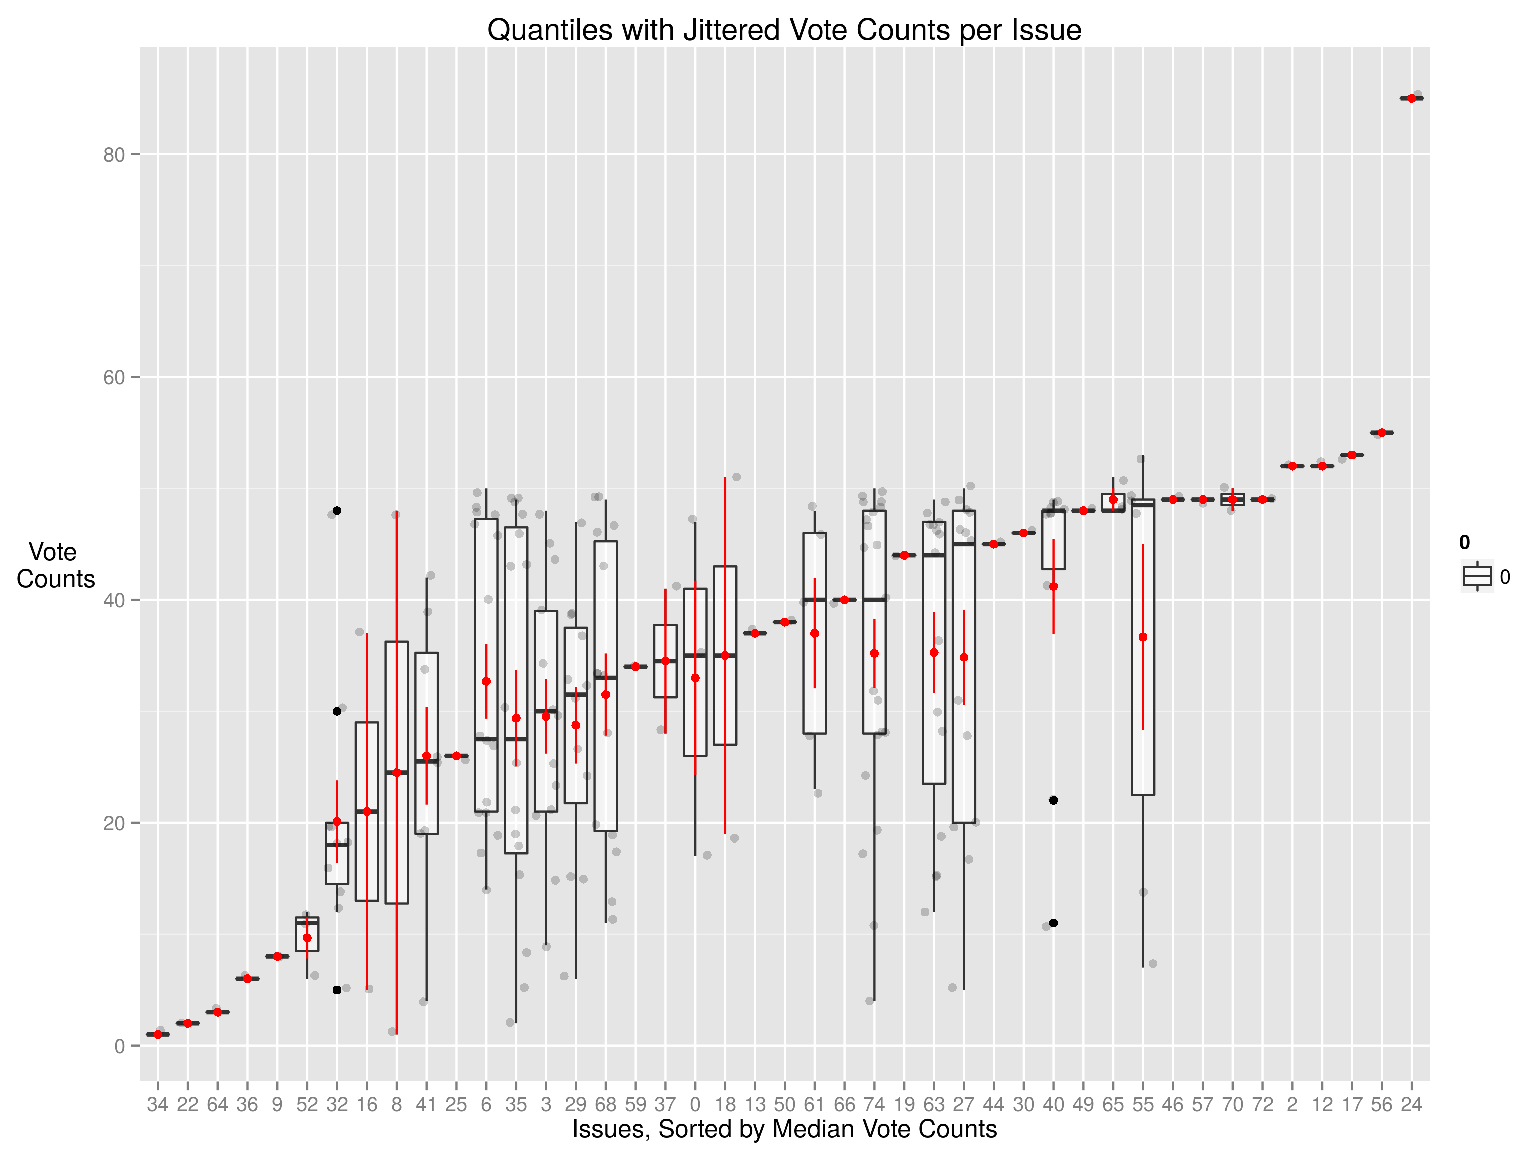
\includegraphics[width=0.49\textwidth]{votes_byIssue.eps}
 \caption[ ]{Summary of proposals, aggregated by issue identifier for an individual session history}
 \label{sessionhistory}
\end{wrapfigure}

Some attributes of this plot deserve attention. 
Notice that the number of votes an issue receives is not determined by the number of times it is considered and that the mean and median values often differ. 
This can be explained by the path-dependent structure of the model, as bills based on a particular issue are not always proposed by the same congress member and by extension may be modified by a different local network or committee before going to the floor for vote.

Individual session histories vary, even with the same experiment parameters. 
This is because each legislative session generates a unique network of ties between congress members. 
The shape of the congressional networks are based on experiment parameters. 
The bifurcated network diagram above (Figure \ref{smallworldnetwork}) is typical of networks with a small number of unaffiliated members (5\%) and roughly equal number of Yellow and Green party members. 
Networks with no party affiliation are more uniform, as are networks with a super-majority.  

We can verify that the model network (at least in with these parameters) can be described as a small world network by calculating some measures of \textit{small-worldness}. 
We use the qgraph implementation \parencite{ec12} of Humphries's methods \parencite{hg08} on our sample network (Appendix, Table \ref{smallworlness}). 
Using Humphries's small-worldness metric as the primary parameter, a network with a value \textgreater 1 can be considered a small world network, though a value \textgreater 3 would be definitive. 
Having global values for network transitivity and average path length higher than for a high number of random sub-networks is another indicator of small-worldness, according to Humphries. 
Our sample network is more typical of real-world networks in the U.S. Congress than the networks we generate with a large super-majority (75\% or 100\% membership of affiliated members in one party) or those experiments without any party affiliation. 

The parameters reflected the sample legislative session history and the sample network are characterizations of typical, observed legislatures. 
However, a key goal of our experiments was to test the relevance of these characteristics on organizational performance.  
Figure \ref{newlaws} shows the number of new laws passed in each of the 30 iterations across the parameter space. 
Notice that in 11 of the 24 experiment jobs in the parameter space, the median number of new laws approved by the congress is zero.
This occurs when there are no externally-defined priorities around which to organize, such as state priorities or party priorities.

\begin{wrapfigure}{l}{0.5\textwidth}
% \vspace{4.5cm}
  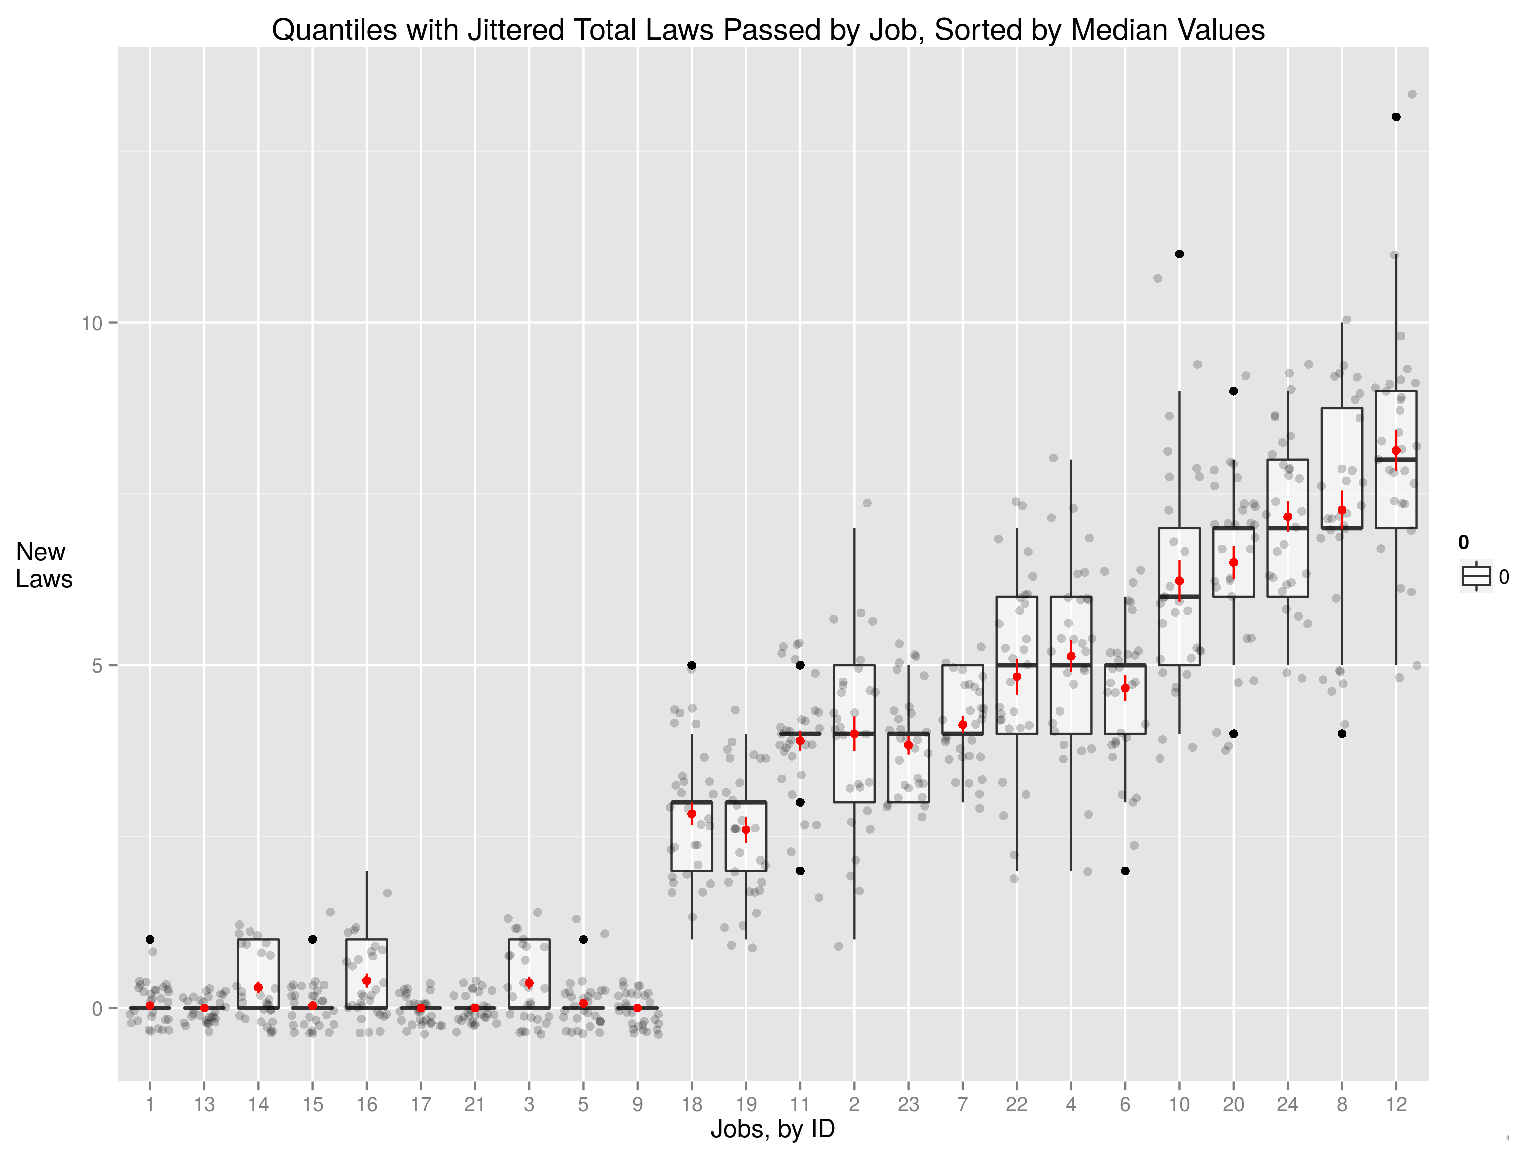
\includegraphics[width=0.49\textwidth]{laws_byJob_jitterQuants.eps}
 \caption[ ]{Some parameters produce no or few new laws in most legislative sessions---typically, when there are no externally-defined priorities.}
 \label{newlaws}
\end{wrapfigure}

We expected that having some key, national issues (state issues) and having some issues aligned with a particular ideology (ideology issues) could influence the productivity (number of laws passed) by each legislative session. 
Our results show that these parameters were not deterministic, except for a condition where there were no state priority issues and no ideology issues.
In those cases there were typically few or no laws passed. 
To be more specific, state priority issues and party ideology issues are defined external to the agents. 
Figure \ref{bypriority} shows the experiment jobs divided by those with or without five state priorities (top facet) and with or without five ideology-related issue priorities. 
Ideology-based issue priorities generated more new laws on average than state priority-based issues. 
Where there are common priorities among members, more bills garner enough support to become laws. 

\begin{wrapfigure}{r}{0.5\textwidth}
% \vspace{4.5cm}
  \includegraphics[width=0.49\textwidth]{laws_byJob_byPriority_jitterQuints.eps}
\caption[ ]{Model runs with no ideology issues and no state priorities consistently produce no new laws, but other structural conditions may also produce no laws.}
 \label{bypriority}
  \vspace{-1cm}
\end{wrapfigure}

The analysis from this point forward excludes the eleven cases where no laws were typically passed, which means that there are no cases in which there are neither state priority issues nor ideology issues. 
In these remaining thirteen cases only two represent cases with a small unaffiliated community and a legislature equally divided between the two parties. 
While the other cases may be interesting, they did not produce sufficient data for analysis.

In the remaining cases we observe a significant difference in the dynamic in the number of new laws, the aggregate number of votes and in the overall satisfaction of the legislatures from modifying bills with additional issues.
Notice three primary characteristics of the cases portrayed in Figures \ref{numlaws}, \ref{numvotes} and \ref{satisfaction}. 
In each of these plots, the top ribbon has five rows, which indicate---from top-to-bottom---the experiment job identifier number, the number of state priorities (zero or five), the number of ideology (party) issues (zero or five), the percentage of Unaffiliated members in the congress and the percentage of Green party members in the congress.
First, the number of provisions required to garner votes may spread across the entire x axis, be all on the left side or all on the right. 
Secondly, the magnitude of the period representing the difference in number of laws passed within a particular case is consistently similar across the cases; regardless of other parameters. 
Finally, the number of laws passed when there is no super-majority is positively correlated with the addition of issues to improve the fit of a particular bill to the reviewers, committee and the floor. 
In other words, when there is a super-majority (at 75\% or 100\% of affiliated members), appeasement decreases the chances that a bill will pass the floor vote.


\begin{figure}%{l}{0.5\textwidth}
% \vspace{-1cm}
 \centering
  \includegraphics[width=0.78\textwidth]{main_laws_prov_byJob.eps}
\caption[ ]{Of those parameters that \textit{usually} produce new laws, the number of laws passed by bundling issues may be either positively or negatively correlated, depending on whether the super-majority is partisan or unaffiliated.}
% \vspace{-.5cm}
 \label{numlaws}
\end{figure}

The phenomena associated with the number of laws that get passed is reflected also in the number of votes bills receive at the floor, though the correlation is not identical. 
For example, notice the case on the far right side---the case represented by job 24---the number of laws passed is positively correlated with additional issues, whereas the total number of votes is negatively correlated with additional issues. 


\begin{figure}%{l}{0.5\textwidth}
% \vspace{-.5cm}
 \centering
  \includegraphics[width=0.78\textwidth]{main_votes_prov_byJob.eps}
\caption[ ]{Of the parameters that \textit{usually} garner votes, party affiliation plays a similar role as for the number of laws passed when bills are augmented with additional issues.}
 \label{numvotes}
\end{figure}

\begin{figure}%{r}{0.5\textwidth}
% \vspace{4.5cm}
 \centering
  \includegraphics[width=0.78\textwidth]{main_sat_prov_byJob.eps}
\caption[ ]{The correlation of overall satisfaction of bills as new issues are added is consistent neither with number of laws passed nor with votes garnered, but still may align with presence of a super-majority.}
 \label{satisfaction}
\end{figure}

The final plot shows a radical departure from the trend with the number of new laws and the total number of votes for an issue. 
In all cases, except that depicted in job 2, adding issues to improve fit decreases overall satisfaction with the bill. 
Even in this case with a small unaffiliated community and a balanced legislature, the correlation looks tenuous. 
If we discount the two lowest values for satisfaction, the correlation will likely tilt to a negative slope. 


\section{Conclusions and Future Work}
This paper has presented a simulated annealing model of policy-formation in Congress. 
Our results indicate that, as more issues are added to a bill, overall legislator satisfaction decreases, regardless of the party structure in a congress. 
Adding issues to appease a minority garners fewer votes and decreases both productivity and overall satisfaction. 
Finally, some structures are not likely to produce legislation, regardless of other factors involved. 

These results suggest several interesting extensions for future research regarding network structures and individual preferences. 
The structure of parties in our simulated legislature could be expanded, to provide a point of comparison with other, more diverse party systems; \textit{e.g.}, proportional representation systems, with many small parties.  
Further investigations of the relationship between legislator preferences and network formation might generate interesting results. 
These two factors seem to be fundamental to the ability of legislators to form effective coalitions.
Varying initial conditions for legislator preferences, perhaps in conjunction with experimental alterations of party structures, could produce a better understanding of the impact of networks on legislation.
Future research might also search for the extent to which a lack of party affiliation changes productivity (number of new laws) or efficiency (number of additional issues required to garner a vote) or a tipping point at which the correlation switches from positive to negative.
We could also extend the model to examine the chances of a bill being passed, depending on which fraction of the membership proposes it: might a bill have better chances of succeeding if a member has a co-sponsor from another party propose the legislation?

Future work could integrate real-world network and preference data into the model. There is an increasing wealth of data on connections between legislators in a variety of deliberating bodies, ranging from national legislatures to smaller local councils. This data might be leveraged to test predictions regarding the impact of party strength and network structure on legislative productivity. It would be worthwhile to collect network metrics for each legislative session and test for correlation between these deeper network characteristics and productivity and efficiency.

Model outputs indicate that legislatures with strong party structures are more productive than legislatures with weak parties. 
This finding is consistent with extant literature regarding emergence of parties in the U.S. Congress as solutions to the collective action problem of generating legislative productivity \parencite{a95}. 
Our model suggests that partisanship is not necessarily an impediment to productivity;  contrary to pundit complaints that excessive partisanship has harmed legislative productivity. 
Our model suggests that incremental appeasement might be impeding Congress's ability to produce legislation.
It is increasingly taken for granted that Congress is destroying itself with partisanship.  
This paper suggests that other factors might actually be the cause of Congress's apparent dysfunction.

\newpage
\appendix
\section*{Technical Appendix} 
\label{App:appendixA}

\subsection*{Technical Details for Generating Leglislator's Positions and Priorities}
 
Starting with element 0 in this priority issues list and proceeding to the end of the list (element $N-1$, where $N = nparty + nstate$), a priority $2*(i + 1)$ is initially assigned to each issue issue.  
Thus, the lowest priority issue will be assigned an initial priority of $2$, and the highest priority issue will be assigned an initial value of $2 * N$.  
All remaining issues ($Num\_of\_Issues - N$) are assigned an initial priority of 1.  
The simulation processes issues incrementally over ${Num\_of\_Issues}^2$ iterations, with the issue to be incremented at each iteration chosen at random according to the probability density of priorities in that iteration.  
Finally, priorities are normalized to the range $[0,1]$.


\begin{table}
 \caption{Fixed and Free Simulation Parameters}
 \begin{tabular}{lp{3.75in}c}
 \hline\noalign{\smallskip}
 Parameter & Description & Value [Variation] \\
 \noalign{\smallskip}
 \hline
 \noalign{\smallskip}
 \texttt{Num\_of\_Representatives} & Size of the legislative body. & 100 \\
 \texttt{Num\_of\_Issues} & Size of the problem set. & 75 \\
 \texttt{Solution\_Bit\_Length} & Bit string length of positions and solutions. & 4 \\
 \texttt{Committees\_Per\_Legislator} & Legislator committee membership; lowest priority issue legislator serves on committee for. & 4 \\
 \texttt{Satisfaction\_Threshold} & Minimum satisfaction a legislator must have with a bill to support it.  A calibrated value but after calibration was fixed for experiment variations. & 0.675 \\
 \texttt{Friend\_Threshold} & Minimum homophily (range [-1,1]) for legislators to be considered for preferential attachment. & 0 \\
 \texttt{Minimum\_Friends} & The number of links added as each legislator is added to the network. & 5 \\
 \texttt{Unaffilitated\_Fraction} & Fraction of the legislative population with no ideological party  affiliation. & [0.05, 0.5, 1.0] \\
 \texttt{Green\_Fraction} & Fraction of the party-affiliated population belonging to the Green party. Remainder belong to the Yellow party. & [0.5, 0.75, 1.0] \\
 \texttt{Ideology\_Issues} & Ideological platform issues for the parties. & [0, 5] \\
 \texttt{State\_Priorities} & High-priority issues for all legislators. & [0, 5] \\
 \hline
 \end{tabular}
 \label{params}
\end{table}

\begin{table}
 \caption{Aggregate metrics recorded for each simulation realization.}
 \begin{tabular*}{1.0\textwidth}{lp{5in}}
 \hline\noalign{\smallskip}
 Output & Description or Note \\
 \noalign{\smallskip}
 \hline
 \noalign{\smallskip}
 Proposals & In rare instances, the legislative body passed laws on all issues in the problem space before the simulation run time.  This metric allowed capture of those instances. \\
 laws count & How many bills were passed into law. \\
 Provisions & How many issues were passed into law. \\
 total satisfaction & Final legislative body satisfaction with all legislation. \\
 total change & Average change in the main issue's positions from proposal to law \\
 total votes & How many votes were cast `aye' over the simulation run. \\
 \hline 
 \end{tabular*}
 \label{metrics}
\end{table}

\begin{table}
 \caption{Measures of ``small-worldness'' with qgraph for our sample, Network 5.}
 \begin{tabular*}{1.0\textwidth}{lcc}
 \hline\noalign{\smallskip}
 Metric & & Value \\
 \noalign{\smallskip}
 \hline
 \noalign{\smallskip}
 "small-worldness" metric & & 1.41070182 \\
 global transitivity & &  0.17755857 \\
 mean transitivity from 300 random sub-nets & & 0.11282573 \\
 lower quantile transitivity, 300 random sub-nets & & 0.09678792 \\
 upper quantile transitivity, 300 random sub-nets & & 0.12978730 \\
 average shortest path & & 2.52565657 \\
 average shortest path, 300 random sub-nets & & 2.26399798 \\
 low quantile shortest path, 300 random sub-nets & & 2.24493232 \\
 upper quantile shortest path, 300 random nets & & 2.28454646 \\
 \hline 
 \end{tabular*}
 \label{smallworlness}
\end{table}

\printbibliography


\end{document}